\documentclass[12pt,a4paper]{report}
\usepackage[utf8]{inputenc}
\usepackage[T1]{fontenc}
\usepackage[french]{babel}
\usepackage{graphicx}
\usepackage{geometry}
\usepackage{setspace}
\usepackage{hyperref}
\usepackage{titlesec}
\usepackage{xcolor}
\geometry{margin=2.5cm}
\usepackage{array}
\usepackage[none]{hyphenat}
\usepackage{float}
\usepackage{makecell}


\onehalfspacing

\titleformat{\chapter}[display]
{\normalfont\bfseries\huge}{\chaptername\ \thechapter}{20pt}{\Huge}
\titleformat{\section}
{\normalfont\Large\bfseries}{\thesection}{1em}{}

\begin{document}
	\pagestyle{empty} 
	\pagenumbering{gobble}  % supprime la numérotation complètement
	
	\chapter*{Liste des abréviations}
	
	\begin{table}[htbp]
		\centering
		\begin{tabular}{|l|l|}
			\hline
			\textbf{Abréviation} & \textbf{Désignation} \\
			\hline
			API & Application Programming Interface \\
			\hline
			CPU & Central Processing Unit \\
			\hline
			HTTP & Hypertext Transfer Protocol \\
			\hline
			IDE & Integrated Development Environment \\
			\hline
			JPA & Java Persistence API \\
			\hline
			LLM & Large Language Model \\
			\hline
			PDF & Portable Document Format \\
			\hline
			RAG & Retrieval-Augmented Generation \\
			\hline
			SARL & Société À Responsabilité Limitée \\
			\hline
			SQL & Structured Query Language \\
			\hline
			UML & Unified Modeling Language \\
			\hline
		\end{tabular}
		\label{tab:liste-abréviations}
	\end{table}
	
	\thispagestyle{empty}
	
	\listoffigures
	\thispagestyle{empty}   % supprime le numéro de page de cette page
	
	\listoftables
	\thispagestyle{empty}
	
	\tableofcontents
	\thispagestyle{empty}
	
	\clearpage
	\pagestyle{plain}
	\pagenumbering{arabic}
	
	\chapter{Contexte du Projet}
	
	\section{Projet de Fin d’Études}
	
	Dans le cadre de notre formation en Génie Informatique à l’École des Hautes Études d’Ingénierie d’Oujda (EHEIO), nous devons réaliser un Projet de Fin d’Études (PFE), visant à consolider et approfondir les compétences acquises durant notre parcours. Ce stage représente une étape cruciale, permettant de transposer les connaissances théoriques dans un environnement professionnel concret.
	
	L’objectif principal est de se familiariser avec les réalités du marché du travail, particulièrement dans le domaine de l’informatique, en perpétuelle évolution. Ce projet offre ainsi l’opportunité d’appliquer nos acquis académiques à des problématiques réelles, tout en développant une approche pratique et méthodique de la gestion de projets technologiques.
	
	Ce stage s’est déroulé dans une entreprise adoptant une méthodologie Scrum, l’une des approches Agile les plus répandues dans le secteur informatique. Cette immersion professionnelle a été l’occasion découvrir le fonctionnement d’une équipe projet en conditions réelles, d'appliquer les principes Agile (itérations, sprints, réunions quotidiennes) dans un cadre professionnel, et de collaborer avec des experts et assimiler les bonnes pratiques en gestion de projets logiciels.
	
	L’utilisation de Scrum a renforcé ma compréhension des processus modernes de développement, tout en améliorant mes capacités d’adaptation et de travail en équipe. Cette expérience a été déterminante pour affiner ma vision du métier d’ingénieur informatique et préparer mon intégration dans le monde professionnel.
	
	Dans ce chapitre, nous commencerons par présenter l’entreprise d’accueil, avant de procéder à une description détaillée des besoins du projet. Cette description comprendra l’identification du problème posé, l’analyse des besoins fonctionnels et non fonctionnels, ainsi que les solutions envisagées pour y répondre.
	
	\section{Entreprise d’accueil}
	
	Ce stage a été réalisé au sein de l’entreprise Algolus, située à Oujda, spécialisée dans les solutions innovantes en intelligence artificielle. Démarré le 24 février 2024, il m’a permis de m’immerger dans un environnement professionnel exigeant, où j’ai pu collaborer avec des experts en IA et en ingénierie logicielle.
	
	\begin{figure}[H]
		\centering
		
\includegraphics[width=0.3\textwidth]{algolus-logo.png}
		\caption{\textit{Logo de Algolus}}
		\label{fig:algolus-logo}
	\end{figure}
	
	\subsection{Description de l’entreprise}
	
	Algolus est une agence web marocaine, créée en 2020, spécialisée dans la conception et le développement de solutions informatiques adaptées aux besoins des clients. Elle s'engage à offrir à ses clients une communication en ligne efficace et sur mesure.

	Ses prestations incluent :
	
	\renewcommand{\labelitemi}{$\bullet$}
	\begin{itemize}
		\item Création et gestion de sites web (dynamiques, statiques, e-commerce, CMS)
		\item Développement d'applications web (mode hybride)
		\item Stratégie digitale complète : infographie, publicité en ligne, marketing digital, community management, E-réputation.
	\end{itemize}
	
	\subsection{Fiche technique de l'entreprise}
	
	Le tableau 1.1 récapitule la fiche technique de l'entreprise Algolus :
	
	\begin{table}[htbp]
		\centering
		\caption{\textit{Fiche technique de l'entreprise Algolus}}
		\begin{tabular}{|l|l|}
			\hline
			\textbf{Dénomination sociale} & Algolus \\
			\hline
			\textbf{Date de création} & 07/10/2020 \\
			\hline
			\textbf{Forme juridique} & SARL \\
			\hline
			\textbf{Capital} & 100.000 Dh \\
			\hline
			\textbf{Chiffre d'affaires} & Indisponible \\
			\hline
			\textbf{Activités} & Développement informatique et marketing digital \\
			\hline
			\textbf{Effectif} & 10 \\
			\hline
			\textbf{Dirigeant} & Radwane BERAHIOUI \\
			\hline
			\textbf{Coordonnées} & \makecell[l]{+212 6644 35967 \\ Redwan.Berahioui@algolus.ma \\ www.algolus.ma \\ IMMEUBLE OUASSIM, Bd Mohammed VI, Oujda 60000} \\
			\hline
		\end{tabular}
		\label{tab:fiche-technique-algolus}  % Pour référence avec \ref
	\end{table}
	
	\subsection{Organigramme de l’entreprise}
	
	La figure 1.2 présente l'organigramme de l'entreprise Algolus :
	
	\begin{figure}[H]
		\centering
		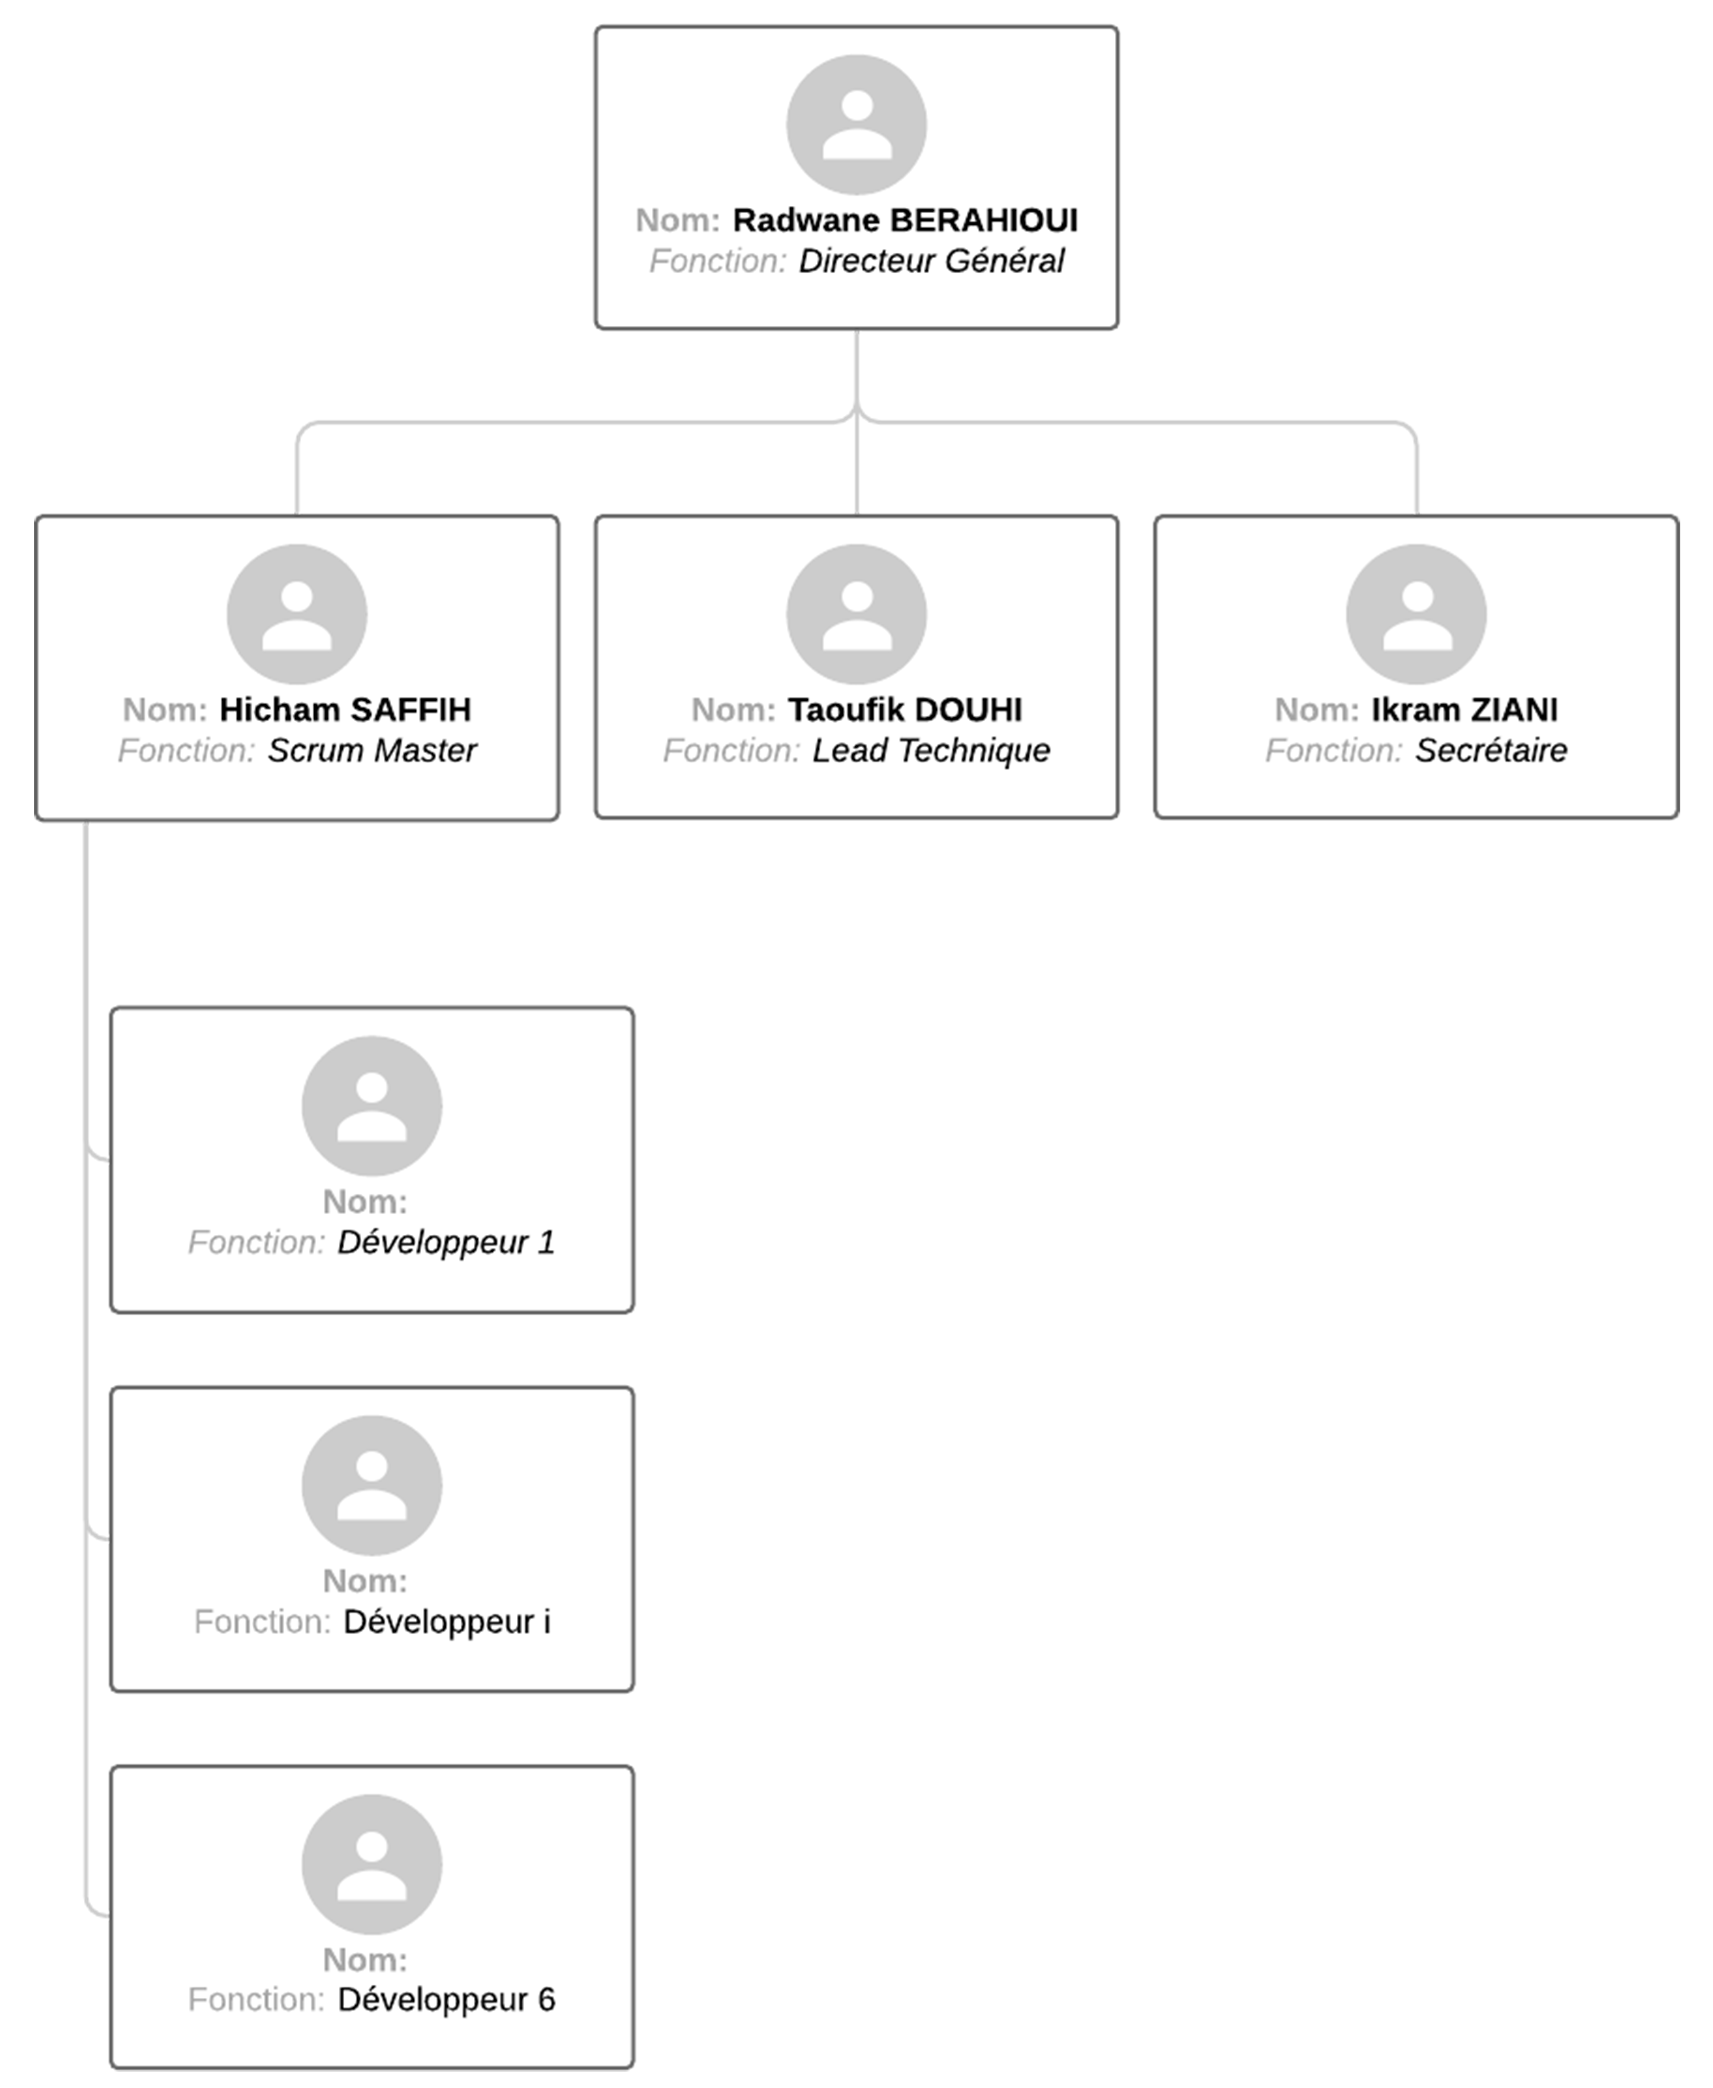
\includegraphics[width=1\textwidth]{algolus-organigramme.png}
		\caption{\textit{Organigramme de l'entreprise Algolus}}
		\label{fig:algolus-organigramme}
	\end{figure}
	
	\section{Description des besoins}
	
	\subsection{Problème}
	
	Dans le cadre du développement logiciel la détection et la correction des erreurs représentent un défi majeur, notamment en raison de la diversité des sources d’anomalies (logs, stack traces, captures d’écran, retours utilisateurs, etc.) et de la complexité croissante des applications. Les méthodes traditionnelles de débogage reposent souvent sur une analyse manuelle, ce qui est chronophage et sujet à des erreurs humaines. De plus, les solutions existantes peinent à offrir une approche générique et intelligente pour interpréter ces anomalies et proposer des correctifs pertinents.
	
	Ce défi prend une dimension particulière dans le cadre des activités de Algolus. La complexité des systèmes gérés par l'entreprise amplifie les difficultés de diagnostic des anomalies. Les équipes techniques consacrent actuellement un volume considérable de leurs ressources temporelles à l'analyse manuelle des incidents, retardant d'autant les mises en production. Par ailleurs, la variété des clients et des cas d'usage entraîne une hétérogénéité des remontées d'erreurs (rapports techniques détaillés pour les clients corporate vs. simples captures d'écran pour les utilisateurs finaux), ce qui rend inefficaces les outils de monitoring conventionnels utilisés jusqu'à présent. Ce constat a motivé l'entreprise à explorer des solutions d'IA générative capables d'unifier l'interprétation des anomalies.
	
	\subsection{Les besoins fonctionnels}
	
	Les besoins fonctionnels définissent les actions spécifiques que le système doit accomplir pour répondre aux exigences métier. Ils décrivent le "quoi", qu'est ce que le système doit faire, sous la forme de fonctionnalités concrètes, de processus et d'interactions avec l'utilisateur. Ces exigences sont formulées par les parties prenantes, à savoir les clients, les utilisateurs, et l'équipe produit, et servent de base à la conception des cas d’usage et des scénarios de test.
	
	Pour garantir que le système de diagnostic d’erreurs réponde efficacement aux attentes des utilisateurs et des équipes techniques, nous avons identifié les besoins fonctionnels suivants :
	
	\begin{enumerate}
		
		\item \textbf{Collecte et Pré-traitement des Données} : Extraction automatique des erreurs et des anomalies des systèmes à partir de :
		stacktraces, parsing des logs, captures d’écran, retours utilisateurs.
		
		\item \textbf{Analyse et Compréhension} : Analyse sémantique de retours d’erreurs, enrichissement contextuel : requêtage d’une base de connaissances (documentation technique, correctifs historiques) via RAG (Retrieval-Augmented Generation).
		
		\item \textbf{Génération de Solutions} : Explication en langage naturel des causes racines, génération de correctifs (ex: snippets de code, étapes de résolution).
		
		\item \textbf{Interfaces utilisateurs} : Soumission des erreurs via des formulaires web pour uploader des stacktraces et des captures d'écran, visualisation des résultats : Dashboard interactif (erreurs en cours, historiques, statistiques).

	\end{enumerate}
	
	\subsection{Les besoins non fonctionnels}
	
	Les besoins non fonctionnels caractérisent le "comment", c'est à dire comment le système doit fonctionner, en précisant ses contraintes de qualité, de performance et d’infrastructure. Contrairement aux besoins fonctionnels, ils ne décrivent pas des fonctionnalités mais des critères tels que la rapidité, la sécurité, la scalabilité ou la facilité de maintenance. Leur respect est essentiel pour assurer la robustesse et l’efficacité du système en conditions réelles.
	
	Pour garantir une intégration harmonieuse dans l’écosystème existant et une expérience utilisateur optimale, les besoins non fonctionnels suivants ont été définies :
	
	\begin{enumerate}
		
		\item \textbf{Performances} : Temps de réponse optimisé, et scalabilité : Support de plusieurs requêtes simultanées.
		
		\item \textbf{Intégration et Interopérabilité} : API REST : Endpoints standardisés et format de réponse avec schéma cohérent, support offline : fonctionnement local avec Ollama.
		
		\item \textbf{Sécurité et Confidentialité} : Protection des données par chiffrement des échanges et anonymisation des logs utilisateurs (RGPD), et authentification : JWT pour l’accès aux APIs sensibles.	
		
		\item \textbf{Expérience Utilisateur} : Ergonomie : interface intuitive, Dark/Light mode et thèmes accessibles.

		
	\end{enumerate}
	
	\subsection{Solutions envisagées}
	
	Ce projet vise à développer une application intelligente et modulaire permettant de détecter et de corriger automatiquement les anomalies logicielles. Les objectifs spécifiques incluent :
	
	\renewcommand{\labelitemi}{$\bullet$}
	\begin{itemize}
		\item Détection avec un taux de réussite d'au moins 80\% les anomalies logicielles sur des sources multimodales.
		
		\item Proposition automatique des correctifs pertinents dans plus de 70\% des cas.
		
		\item Optimisation du temps moyen de résolution d’erreurs de 30\% par rapport aux méthodes manuelles.
	\end{itemize}
	
	Pour atteindre ces objectifs, le projet s’appuie sur une architecture innovante :
	
	\begin{enumerate}
		\item \textbf{Analyse Multimodale des Erreurs} : Implémenter un système capable d’interpréter des données hétérogènes (stack traces, logs texte, captures d’écran, etc.), et utiliser des techniques de RAG pour enrichir les requêtes avec une base de connaissances (documentation technique, résolutions d’erreurs courantes).
		
		\item \textbf{Génération Automatique de Correctifs} : Exploiter des LLMs (via Ollama) pour suggérer des corrections précises et contextualisées.
		
		\item \textbf{Intégration et Scalabilité} : Développer un backend Spring Boot flexible, couplé à LangChain4J pour orchestrer les appels IA, et un système de gestion de base de données qui prend en charge les bases de données vectorielles, comme PostgeSQL, et permettre une extension future via des connecteurs pour différents outils de monitoring.
		
		\item \textbf{Optimisation et Évaluation} : mesurer l’efficacité du système via des métriques de précision (taux de détection, pertinence des correctifs), et effectuer un Benchmark : comparaison sur des jeux de données communs.
		
	\end{enumerate}
	
	\chapter{Analyse fonctionnelle et modélisation}
	
	\section{Importance de l'analyse fonctionnelle}
	
	L’analyse fonctionnelle constitue une étape clé dans tous projets de développement informatique, car elle permet de bien comprendre les besoins du client et les contraintes du système à réaliser. Elle sert à identifier les fonctionnalités attendues, à détecter les éventuelles incohérences et à poser les bases d’une conception solide. Une analyse fonctionnelle bien menée réduit considérablement les risques d’erreurs en phase de développement, facilite la planification du travail et améliore la qualité globale du produit final, ce qui lui rend essentielle pour assurer la réussite du projet.
	
	Dans ce chapitre nous présentons une introduction à la modélisation UML, en rappelant ses principes fondamentaux et son utilité dans le développement logiciel. Par la suite nous exposerons les différents types de diagrammes utilisés dans notre étude, à savoir le diagramme de cas d’utilisation, les diagrammes de séquences, ainsi que le diagramme de classes.
	
	\section{Unified Modeling Language}
	
	Dans le cadre d’un projet de développement informatique la modélisation UML (Unified Modeling Language) joue un rôle essentiel en facilitant la compréhension, la conception et la communication autour du système à développer. UML propose un ensemble de diagrammes normalisés qui permettent de représenter visuellement les différentes dimensions d’un logiciel, telles que la structure, le comportement et les interactions entre les composants.
	
	L’utilisation des diagrammes UML comme les diagrammes de cas d’utilisation, de classes et de séquences permet de clarifier les besoins fonctionnels et non fonctionnels dès les premières phases du projet, de favoriser une meilleure communication entre les développeurs, les analystes et les clients, de détecter de façon précoce les incohérences ou erreurs potentielles dans la conception, et aussi de servir de documentation technique structurée pour le développement, les tests et la maintenance future du logiciel.
	
	Ainsi, UML constitue un outil précieux pour assurer la qualité, la cohérence et la pérennité d’un projet informatique, en apportant une vision globale et partagée du système.
	
	\section{Diagramme de cas d'utilisation}
	
	\subsection{Définition}
	
	Un diagramme de cas d'utilisation est une représentation visuelle des interactions entre les acteurs (utilisateurs, systèmes) et les fonctionnalités d'une application. Il identifie les besoins métiers sous forme d'actions (cas d’utilisation) et montre qui fait quoi, sans entrer dans les détails techniques.
	
	\subsection{Acteurs}
	
	Dans un diagramme de cas d'utilisation, les acteurs sont les entités qui interagissent avec le système pour accomplir un objectif précis. Un acteur peut être primaire (s'il est déclencheur d'un cas d'utilisation) ou secondaire (intervient dans un cas d'utilisation mais ne le déclenche pas). D'une autre part, un acteur peut être humain ou bien un acteur système.
	
	Trois types d'acteurs sont impliqués dans notre cas :
	
	\begin{itemize}
		\item \textbf{Utilisateur} : peut être un développeur ou un testeur qui rapporte une erreur, et peut interagir via une API REST ou bien une interface web.
		
		\item \textbf{Administrateur du système} : responsable de la mise à jour des connaissances du système et de la configuration des modèles.
		
		\item \textbf{Système} : le moteur de traitement intelligent, responsable d'analyser les anomalies, et de proposer des correctifs appropriés.
	\end{itemize}
	
	\subsection{Diagramme de cas d'utilisation}
	
	La figure \ref{fig:use-case} présente le diagramme de cas d'utilisation de notre application :
	
	\begin{figure}[H]
		\centering
		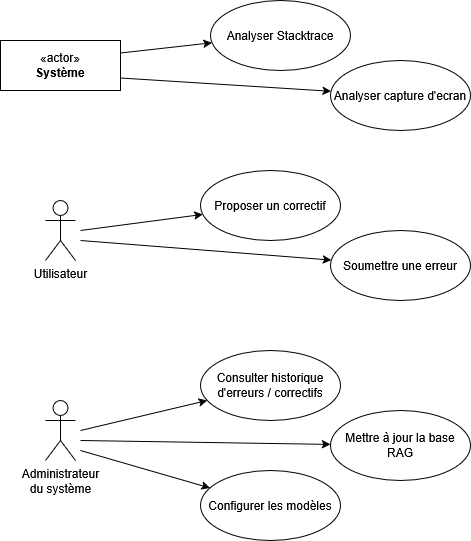
\includegraphics{use-case.drawio.png}
		\caption{\textit{Diagramme de cas d'utilisation}}
		\label{fig:use-case}
	\end{figure}
	
	\section{Diagrammes de séquences}
	
	\subsection{Définition}
	
	Un diagramme de séquences est un type de diagramme UML, utilisé pour modéliser les interactions entre les différents objets ou composants d'un système dans un scénario précis. Il met en évidence l'ordre chronologique des messages échangés entre les acteurs et les objets, les interactions dynamiques entre les éléments du système, et la durée de vie des objets participant au scénario.
	
	\subsection{Diagramme de séquences principal}
	
	Cette application d'analyse d'erreurs techniques repose sur une architecture modulaire, où chaque composant joue un rôle précis dans le traitement des requêtes. Voici une présentation des éléments clés qui permettent au système de comprendre, contextualiser et répondre aux problèmes soumis par les utilisateurs :
	
	\begin{itemize}
		
		\item \textbf{Utilisateur} : L'Utilisateur constitue le point de départ du système. Ce composant représente l'acteur humain qui interagit avec l'application via une interface web ou des appels API. Il soumet des requêtes contenant des stacktraces d'erreur et éventuellement des captures d'écran.
		
		\item \textbf{LLM (Large Language Model)} : Est un modèle d'intelligence artificielle entraîné sur des volumes massifs de données textuelles, capable de comprendre, générer et manipuler du langage naturel de manière contextuelle. Basé sur des architectures de deep learning (comme les transformers), il excelle dans des tâches variées (réponse aux questions, traduction, synthèse de texte, etc.) en prédisant des séquences de mots probabilistes. Contrairement aux systèmes traditionnels, un LLM ne suit pas de règles prédéfinies, mais apprend des motifs linguistiques à partir de ses données d'entraînement.
		
		\item \textbf{RAG (Retrieval-Augmented Generation)} : apporte une dimension documentaire aux analyses. Composé de trois éléments principaux - un modèle d'embedding, un stockage vectoriel et un moteur de recherche - ce pipeline sophistiqué permet d'enrichir les réponses du LLM avec des connaissances provenant d'une base documentaire technique. Le processus transforme d'abord les requêtes et documents en vecteurs, puis effectue des recherches de similarité dans le stockage vectoriel avant d'injecter les documents pertinents dans le contexte du LLM.
		
		\item \textbf{Agent AI} : sert de chef d'orchestre principal dans l'architecture. Ce service intelligent coordonne l'ensemble du processus d'analyse. Il reçoit les requêtes brutes de l'utilisateur, les enrichit en combinant plusieurs techniques avancées comme le RAG et la mémoire conversationnelle, puis les présente au modèle de langage sous une forme optimale.
		
		\item \textbf{ChatModel} : incarne le moteur de génération de langage naturel. Ce composant spécifique, configuré pour utiliser des modèles locaux ou externes, transforme les prompts structurés en analyses techniques détaillées.
		
		\item \textbf{ChatMemory} : joue un rôle crucial dans la maintien du contexte conversationnel. Implémentée comme une mémoire à fenêtre glissante, elle conserve les N dernières interactions de chaque session utilisateur, identifiée par un MemoryId unique. Cette mémoire permet au LLM de maintenir une cohérence dans les échanges et de se souvenir des points clés abordés précédemment dans la conversation, essentiel pour les analyses techniques itératives où l'utilisateur affine progressivement sa requête.
		
	\end{itemize}
	
	Le diagramme de séquences dans la figure \ref{fig:ds-ai-agent.drawio} décrit le flux de messages entre ces composants.
	
	\begin{figure}[H]
		\centering
		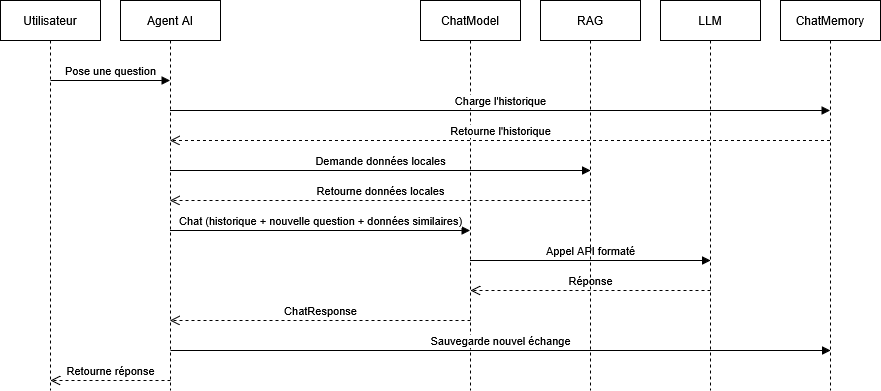
\includegraphics[width=\textwidth]{ds-ai-agent.drawio.png}
		\caption{\textit{Diagramme de séquences décrivant le fonctionnement d'un agent AI}}
		\label{fig:ds-ai-agent.drawio}
	\end{figure}
	
	\subsection{Diagramme de séquences spécifique : RAG}
	
	Nous allons creuser un peu dans les composants du système RAG, voici une énumération de ces composants avec chacun son rôle :
	
	\begin{itemize}
		
		\item \textbf{Resource} : Constitue la matière première du système RAG. Il s'agit de la source originelle des données qui alimenteront la base de connaissances. Ces ressources peuvent prendre diverses formes : fichiers PDF contenant de la documentation technique, pages web de référence, extraits de bases de données, ou tout autre support contenant des informations pertinentes. Le système doit être capable de traiter ces ressources hétérogènes, qu'elles proviennent de systèmes internes ou de sources externes. La qualité et l'actualité des resources déterminent en grande partie l'efficacité finale du système RAG.
		
		\item \textbf{Tokenizer} : Joue un rôle fondamental dans le prétraitement du texte. Ce composant décompose le contenu textuel en unités significatives appelées tokens, qui peuvent correspondre à des mots entiers, des sous-mots ou même des caractères individuels selon la méthode employée. Des algorithmes avancés comme ceux proposés par HuggingFace permettent une tokenisation optimale qui préserve le sens tout en gérant les particularités linguistiques. La tokenisation est cruciale car elle influence directement la qualité des embeddings générés ultérieurement.
		
		\item \textbf{DocumentParser} : Assure la transformation des ressources brutes en documents structurés. Ce composant doit comprendre divers formats de fichiers (PDF, HTML, Markdown, etc.) et en extraire le contenu textuel significatif tout en conservant les métadonnées importantes. Des bibliothèques spécialisées comme sont souvent employées pour cette tâche complexe. Le DocumentParser nettoie également le texte en supprimant les éléments non pertinents (en-têtes, pieds de page, balises HTML) pour ne conserver que l'information essentielle.
		
		\item \textbf{Document} : Représente la forme normalisée et standardisée des informations après traitement. Chaque document contient non seulement le texte brut nettoyé, mais aussi des métadonnées descriptives (titre, auteur, date de création, source) qui faciliteront son identification et son utilisation ultérieure. Un identifiant unique est attribué à chaque document pour permettre son suivi tout au long du pipeline. Cette structuration rigoureuse est essentielle pour maintenir la cohérence des données dans les étapes suivantes du processus RAG.
		
		\item \textbf{EmbeddingModel} : Est au cœur de la transformation sémantique du système. Ce modèle sophistiqué convertit le texte en représentations vectorielles denses (embeddings) qui capturent le sens profond des contenus. Des modèles sont spécialisés dans cette tâche produisent des vecteurs où la similarité spatiale correspond à la similarité sémantique. La qualité de l'EmbeddingModel détermine directement la capacité du système à retrouver des documents pertinents pour une requête donnée.
		
		\item \textbf{EmbeddingStoreIngestor} : Orchestre le processus complet d'indexation des documents. Ce composant supervise plusieurs opérations critiques : il applique la tokenisation et la segmentation des textes, déclenche la génération des embeddings via l'EmbeddingModel, et gère le stockage final dans l'EmbeddingStore. \\ L'EmbeddingStoreIngestor implémente souvent des stratégies de traitement par lots pour optimiser les performances et peut gérer des pipelines complexes de prétraitement avant la vectorisation.
		
		\item \textbf{EmbeddingStore} : Sert de mémoire à long terme au système RAG. Cette base de données vectorielle spécialisée stocke les embeddings générés et permet des recherches rapides de similarité. L'EmbeddingStore doit supporter des opérations massives d'insertion tout en maintenant des temps de réponse faibles pour les requêtes.
		
		\item \textbf{Retriever} : Est le composant qui établit le pont entre les questions des utilisateurs et la base de connaissances. Lors d'une requête, le Retriever transforme d'abord la question en embedding, puis recherche dans l'EmbeddingStore les documents dont les vecteurs sont les plus proches. Ce composant implémente des algorithmes de similarité vectorielle (cosine similarity par exemple) et peut être finement paramétré (nombre de résultats retournés, seuil de similarité minimal). Le Retriever joue ainsi un rôle déterminant dans la pertinence des résultats fournis au LLM.
		
	\end{itemize}
	
	Le diagramme de séquences dans la figure \ref{fig:ds-rag.drawio} résume ce processus.
	
	\begin{figure}[H]
		\centering
		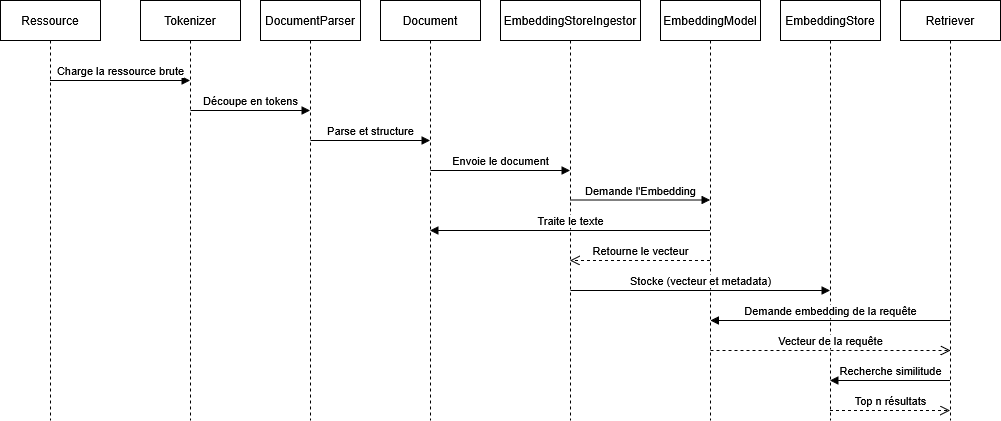
\includegraphics[width=\textwidth]{ds-rag.drawio.png}
		\caption{\textit{Diagramme de séquences décrivant le fonctionnement d'un RAG}}
		\label{fig:ds-rag.drawio}
	\end{figure}
	
	\chapter{Réalisation}
	
	Ce chapitre présente la phase de concrétisation du projet, où les choix techniques et architecturaux se traduisent en une implémentation fonctionnelle. Il décrit l'environnement de développement (outils, frameworks, librairies, etc.), l'architecture logicielle retenue et son adéquation avec les besoins, les défis techniques rencontrés et les solutions apportées, et les composants clés implémentés avec des extraits de code significatifs, et des captures d'écran illustrant les résultats obtenus.

	\section{Stack technique}
	
	\subsection{Langages}
	
	\subsubsection{Java}
	
	\begin{figure}[H]
		\begin{minipage}{0.8\textwidth}
			Java est un langage de programmation orienté objet, robuste et multiplateforme, largement utilisé dans le développement d'applications d'entreprise. Sa forte typographie, sa gestion automatique de la mémoire (via le garbage collector) et son écosystème riche (bibliothèques, frameworks) en font un choix idéal pour les systèmes backend complexes.
		\end{minipage}
		\hfill
		\begin{minipage}{0.15\textwidth}
			\begin{figure}[H]
				\centering
				
\includegraphics[width=\linewidth]{java-logo.png}
				\label{fig:java-logo}
			\end{figure}			
		\end{minipage}
	\end{figure}
		
	\subsection{Frameworks}
	
	\subsubsection{Spring}
	
	\begin{figure}[H]
		\begin{minipage}{0.8\textwidth}
			Spring est un framework modulaire pour Java, simplifiant le développement d'applications grâce à l’inversion de contrôle (IoC) et la programmation orientée aspect (AOP).
		\end{minipage}
		\hfill
		\begin{minipage}{0.15\textwidth} 
			\begin{figure}[H]
				\centering
				
\includegraphics[width=\linewidth]{spring-logo.png}
				\label{fig:spring-logo}
			\end{figure}
		\end{minipage}
	\end{figure}
	
	\subsubsection{Spring Boot}
	
	\begin{figure}[H]
		\begin{minipage}{0.8\textwidth}
			Spring Boot étend Spring en fournissant des configurations automatiques, un serveur embarqué (Tomcat, Netty) et des outils clés en main (Spring Data, Spring Security), permettant de créer des applications standalone rapidement.
		\end{minipage}
		\hfill
		\begin{minipage}{0.15\textwidth} 
			\begin{figure}[H]
				\centering
				
\includegraphics[width=\linewidth]{spring-boot-logo.png}
				\label{fig:spring-boot-logo}
			\end{figure}
		\end{minipage}
	\end{figure}
	
	
	\subsubsection{LangChain4j}
	
	\begin{figure}[H]
		\begin{minipage}{0.8\textwidth}
				LangChain4J est une bibliothèque Java inspirée de LangChain (Python), conçue pour intégrer facilement des LLMs (Modèles de Langage) dans des applications. Elle offre des abstractions pour la gestion des prompts, le RAG, les appels aux modèles (OpenAI, Ollama, etc.), et la connexion à des bases de données vectorielles.
		\end{minipage}
		\hfill
		\begin{minipage}{0.15\textwidth} 
			\begin{figure}[H]
				\centering
				
\includegraphics[width=\linewidth]{langchain4j-logo.png}
				\label{fig:langchain4j-logo}
			\end{figure}
		\end{minipage}
	\end{figure}
	
	\subsection{Bibliothèques}
	
	\subsubsection{Apache Commons}
	
	\begin{figure}[H]
		\begin{minipage}{0.8\textwidth}
			Apache Commons est une bibliothèque Java open-source fournissant des composants réutilisables pour simplifier le développement. Dans ce projet, elle sert à combler des besoins techniques récurrents avec des solutions optimisées et robustes.
		\end{minipage}
		\hfill
		\begin{minipage}{0.15\textwidth} 
			\begin{figure}[H]
				\centering
				
\includegraphics[width=\linewidth]{apache-commons-logo.png}
				\label{fig:apache-commons-logo}
			\end{figure}
		\end{minipage}
	\end{figure}
		
	\subsection{Systèmes de gestion de bases de données}
	
	\subsubsection{PostgreSQL}
	
	\begin{figure}[H]
		\begin{minipage}{0.8\textwidth}
			PostgreSQL est un système de gestion de base de données relationnelle (SGBDR) open-source, robuste et extensible. Dans le cadre de ce projet, il joue un rôle central pour stocker et gérer les données structurées nécessaires au bon fonctionnement de l’application, et fournit des plugins pour l'IA, notamment PgVector, qui gère les bases de données vectorielles.
		\end{minipage}
		\hfill
		\begin{minipage}{0.15\textwidth} 
			\begin{figure}[H]
				\centering
				
\includegraphics[width=\linewidth]{postgresql-logo.png}
				\label{fig:postgresql-logo}
			\end{figure}
		\end{minipage}
	\end{figure}
	
	\subsection{Outils et environnement}
	
	\subsubsection{Ollama}
	
	\begin{figure}[H]
		\begin{minipage}{0.8\textwidth}
			Ollama est un outil open-source permettant d’exécuter localement des LLMs (comme Llama 3, Mistral, Gemma) sans dépendre d’une API externe. Il est idéal pour prototyper des solutions IA offline, contrôler les coûts et la confidentialité des données, et personnaliser finement les modèles via des modelfiles.
		\end{minipage}
		\hfill
		\begin{minipage}{0.15\textwidth} 
			\begin{figure}[H]
				\centering
				
\includegraphics[width=\linewidth]{ollama-logo.png}
				\label{fig:ollama-logo}
			\end{figure}
		\end{minipage}
	\end{figure}
	
	\subsubsection{Maven}
	
	\begin{figure}[H]
		\begin{minipage}{0.8\textwidth}
			Outil de build automatisé pour projets Java, qui gère Les dépendances (téléchargement auto), le packaging (JAR/WAR), et les cycles de compilation/test.
		\end{minipage}
		\hfill
		\begin{minipage}{0.15\textwidth} 
			\begin{figure}[H]
				\centering
				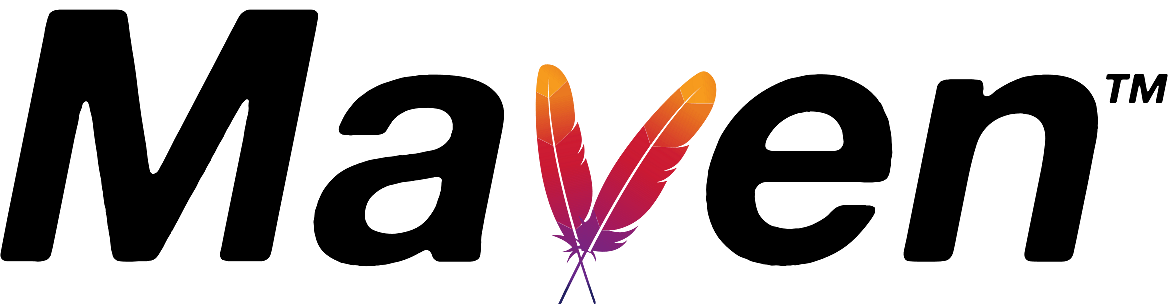
\includegraphics[width=\linewidth]{maven-logo.png}
				\label{fig:maven-logo}
			\end{figure}
		\end{minipage}
	\end{figure}
	
	\subsubsection{IntelliJ IDEA}
	
	\begin{figure}[H]
		\begin{minipage}{0.8\textwidth}
			IntelliJ IDEA est un IDE puissant pour Java/Kotlin, développé par JetBrains. Ses avantages incluent une analyse intelligente du code (suggestions, détection d’erreurs), une intégration native avec Spring Boot et Maven/Gradle, des outils pour le débogage, le profiling et les tests, et des extensions pour l’IA (ex : GitHub Copilot).
		\end{minipage}
		\hfill
		\begin{minipage}{0.15\textwidth} 
			\begin{figure}[H]
				\centering
				
\includegraphics[width=\linewidth]{intellij-logo.png}
				\label{fig:intellij-logo}
			\end{figure}
		\end{minipage}
	\end{figure}
	
	\subsubsection{Git}
	
	\begin{figure}[H]
		\begin{minipage}{0.8\textwidth}
			Git est un système de contrôle de version distribué, essentiel pour le développement collaboratif. Il permet de suivre les modifications du code source, de gérer les branches, et de fusionner les travaux de plusieurs contributeurs. Grâce à des plateformes comme GitHub, il facilite le partage et la revue de code. Son utilisation améliore la traçabilité, la qualité et la productivité dans les projets logiciels.
		\end{minipage}
		\hfill
		\begin{minipage}{0.15\textwidth} 
			\begin{figure}[H]
				\centering
				
\includegraphics[width=\linewidth]{git-logo.png}
				\label{fig:git-logo}
			\end{figure}
		\end{minipage}
	\end{figure}
	
	\section{Architecture technique du projet}
	
	Le projet repose sur une architecture modulaire et évolutive, construite autour des meilleures pratiques du développement Java moderne, de l'IA générative et de l’ingénierie logicielle. Il s’appuie sur les technologies suivantes :
	
	\begin{itemize}
		
		\item \textbf{Spring Boot} : Est le framework retenu pour le développement de la couche back-end. Il s’agit d’un choix stratégique largement justifié par les besoins du projet en termes de performance, de maintenabilité et d’intégration avec des composants d’intelligence artificielle.
		
		Spring Boot permet de structurer l’application de manière modulaire, en séparant clairement les responsabilités (contrôleurs, services, configuration, etc.). Cette organisation favorise une bonne lisibilité du code et facilite son évolution.
		
		L’application est également portable, dans la mesure où elle peut être conditionnée sous forme de JAR exécutable et déployée facilement sur tout environnement compatible Java, sans dépendance à un serveur externe.
		
		Un autre atout majeur est le caractère évolutif de Spring Boot : il s’intègre naturellement avec des bibliothèques telles que LangChain4j ou des bases de données comme PostgreSQL, ce qui permet d’ajouter de nouvelles fonctionnalités (IA, recherche vectorielle, mémoire contextuelle) sans remise en cause de l’existant.
		
		Le framework est aussi testable : il propose des outils natifs pour la réalisation de tests unitaires et d’intégration, garantissant la qualité et la stabilité du code produit.
		
		Enfin, Spring Boot est hautement extensible. Si le projet venait à croître en complexité, il serait tout à fait envisageable de faire évoluer l’architecture vers un modèle microservices avec des outils comme Spring Cloud.
		
		\item \textbf{LangChain4j} : Pour permettre l’analyse intelligente des erreurs à l’aide d’un modèle de langage (LLM), le projet s’appuie sur la bibliothèque LangChain4j, une adaptation Java du framework LangChain initialement développé pour Python. Ce composant joue un rôle central dans l’intégration des fonctionnalités d’intelligence artificielle générative.
		
		LangChain4j facilite la mise en œuvre d’un mécanisme de RAG (Retrieval-Augmented Generation), en combinant génération de texte via un LLM et récupération de documents pertinents à partir d’une base vectorielle. Il s’intègre naturellement avec un modèles de langage, et avec des composants tels que la mémoire de conversation, le modèle d’embedding et le store d’embeddings.
		
		L’utilisation de LangChain4j rend l’application extensible et modulaire, car ses composants (LLM, mémoire, embeddings, etc.) sont interchangeables via des interfaces. Elle offre également un haut niveau de configurabilité, permettant d’adapter dynamiquement les modèles utilisés, la taille de la mémoire contextuelle ou encore les critères de pertinence documentaire.
		
		Enfin, son intégration avec Spring Boot via des beans injectables simplifie grandement sa mise en œuvre dans l’architecture globale du projet. Cela permet d’enrichir les traitements métier avec une couche d’IA tout en conservant la lisibilité et la testabilité du code.
		
		\item \textbf{Ollama} : Pour exécuter les modèles de langage en local sans dépendre de services cloud externes, le projet intègre Ollama, une plateforme légère permettant de servir des LLM open-source tels que Mistral, Llama3 ou Qwen qui offre des versions multimodales. Ollama agit comme un point d’accès HTTP local à un modèle de génération de texte, que LangChain4j peut interroger de manière transparente.
		
		Ce choix présente plusieurs avantages : tout d’abord, il rend l’application autonome et portable, car aucun appel à une API cloud (comme OpenAI ou Hugging Face) n’est requis. Cela permet un déploiement sur des machines locales ou en environnement isolé (on-premise), tout en respectant les contraintes de confidentialité des données.
		
		Grâce à une configuration centralisée (adresse du serveur, modèle utilisé, température, etc.), Ollama est également hautement configurable. Son intégration dans le projet se fait via des beans Spring instanciés dynamiquement dans la classe de configuration (AiConfig), ce qui permet d’adapter ou changer le modèle utilisé sans modifier la logique métier.
		
		Enfin, en travaillant de concert avec LangChain4j, Ollama permet la génération de réponses contextualisées et pertinentes, en tenant compte des documents récupérés et des interactions passées. Cela renforce la capacité de l'application à fournir des analyses d'erreurs enrichies, précises et directement exploitables.
		
		\item \textbf{PostgreSQL} : Utilisé comme système de gestion de base de données relationnelle, avec une orientation spécifique vers le stockage vectoriel, dans le cadre de l’indexation et de la recherche de documents sémantiques. Grâce à l’extension pgvector, PostgreSQL devient capable de stocker des vecteurs d’embedding et d’effectuer des recherches de similarité, essentielles dans une approche RAG (Retrieval-Augmented Generation).
		
		Le choix de PostgreSQL repose sur plusieurs critères clés : sa fiabilité, sa scalabilité et sa maturité en production. En plus de gérer des données relationnelles classiques (logs, utilisateurs, paramètres…), il peut aussi indexer efficacement des vecteurs issus des modèles d’embedding (ex. OllamaEmbeddingModel), et permettre des requêtes de type nearest neighbor search.
		
		Son intégration avec Spring Boot est fluide grâce à JPA ou JDBC, et son usage dans ce projet est évolutif : dans un premier temps, les embeddings sont stockés en mémoire (InMemoryEmbeddingStore), mais la bascule vers PostgreSQL permettra une persistance et une scalabilité bien supérieures, tout en conservant une interface compatible avec les composants LangChain4j.
		
		Ainsi, PostgreSQL joue un rôle fondamental dans la stratégie d’enrichissement contextuel des requêtes utilisateur, en permettant à l’IA de s’appuyer sur des documents pertinents stockés localement de façon fiable et interrogeable.
		
	\end{itemize}
	
	La figure \ref{fig:illustration-graphique} illustre de manière synthétique les interactions entre les principaux composants techniques de l’architecture mise en place dans le cadre de ce projet.
	
	\begin{figure}[H]
		\centering
		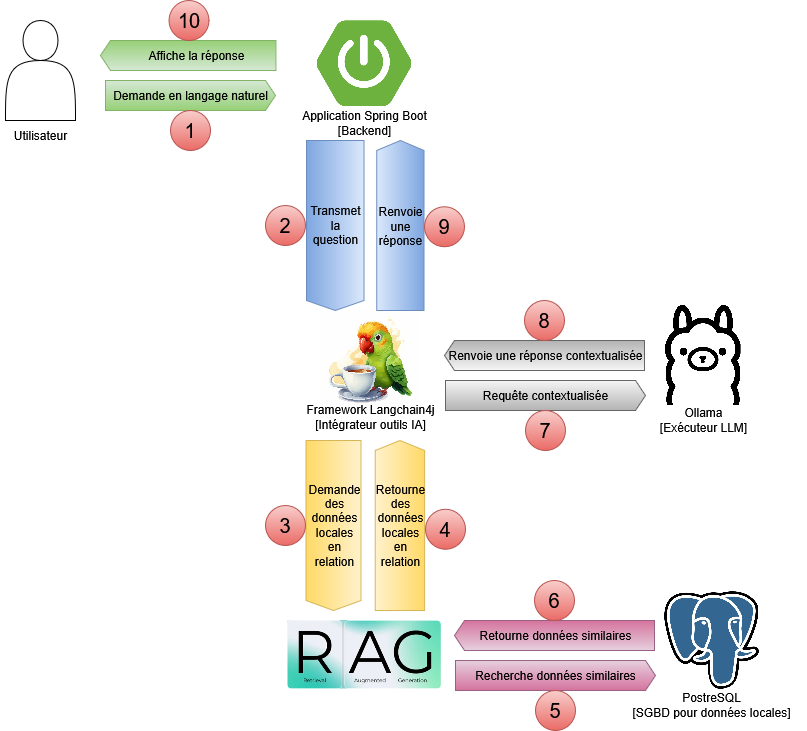
\includegraphics[width=1\textwidth]{illustration-graphique.drawio.png}
		\caption{\textit{Diagramme d'architecture technique}}
		\label{fig:illustration-graphique}
	\end{figure}
	
	\section{Bonnes pratiques appliquées du développement Java}
	
	Dans le développement logiciel, l'adoption de bonnes pratiques de codage est essentielle pour garantir la robustesse, la maintenabilité et l'évolutivité des applications. Un code bien structuré, avec une logique claire et une réduction des redondances, facilite non seulement les futures modifications, mais améliore aussi la collaboration entre développeurs. Cette section aborde des principes clés pour optimiser l'écriture du code, en mettant l'accent sur des méthodes qui en améliorent la qualité tout en réduisant les risques d'erreurs.
	
	\subsection{Utilisation de Bibliothèques Matures : Apache Commons}
	
	Plutôt que de réinventer la roue, il est recommandé d’utiliser des bibliothèques robustes comme Apache Commons, qui fournit des utilitaires optimisés pour plusieurs opérations telles que la manipulation de collections, les opérations sur les chaînes, et les validations.
	
	Pour mettre en lumière les utilisations de ces utilitaires dans notre projet, prenons par exemple la méthode \verb|estimateTokenCountInText(String text)| de la classe \verb|TokenizerMyAppImpl|, dont la figure \ref{fig:before-string-utils} montre une implémentation classique.
	
	\begin{figure}[H]
		\centering
		\fbox{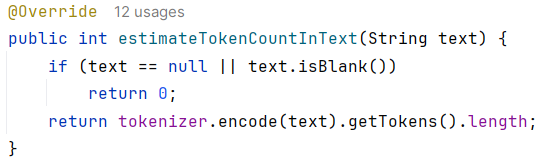
\includegraphics{before-string-utils.png}}
		\caption{\textit{Implémentation sans utiliser Apache Commons}}
		\label{fig:before-string-utils}
	\end{figure}
	
	Cette approche, bien que fonctionnelle, présente plusieurs limitations : la combinaison de deux vérifications dans une même condition, la duplication de cette logique à de nombreux endroits du code, et le risque potentiel de \verb|NullPointerException|.
	
	L'adoption d'une nouvelle implémentation exploitant la bibliothèque Apache Commons est montrée dans la figure \ref{fig:after-string-utils}.
	
	\begin{figure}[H]
		\centering
		\fbox{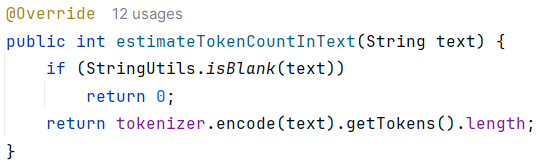
\includegraphics{after-string-utils.png}}
		\caption{\textit{Implémentation en utilisant Apache Commons}}
		\label{fig:after-string-utils}
	\end{figure}
	
	La méthode isBlank() de la classe StringUtils retourne true dans trois cas : si text est null, ou une chaine de caractères vides, ou une chaine de caractères ne contenant que des espaces blancs, Ce qui donne plus de robustesse au projet, en évitant les NullPointerException sans besoin de vérifier null explicitement, améliore la lisibilité en remplaçant une condition complexe par un seul appel clair, et garantit un comportement uniforme dans tout le projet.
	
	\subsection{Approches de parcours de collections en Java}
	
	Durant le développement, j'ai été amené à manipuler des collections de données. Plusieurs approches s'offraient alors à moi, chacune présentant des caractéristiques distinctes :
	
	\begin{itemize}
		
		\item \textbf{La boucle for traditionnelle} : Approche historique de Java, elle se base sur un index numérique. Bien que simple conceptuellement, elle montre plusieurs limitations : une syntaxe verbeuse nécessitant la déclaration d'un compteur, un risque d'erreurs d'indice (\verb|IndexOutOfBoundsException|), une inadaptation aux structures non indexées comme les Set, et une difficulté à maintenir pour des traitements complexes.
		
		\item \textbf{La boucle for-each} : Introduite dans Java 5, elle simplifie le parcours, en offrant une syntaxe plus concise et plus lisible, et en éliminant le risque d'erreurs d'indice, cependant elle ne permet pas de modification concurrente, en plus d'être limitée à un parcours séquentiel simple.
		
		\item \textbf{L'Iterator} : Fournit un contrôle fin sur le parcours, en effet, il permet la suppression d'éléments (méthode \verb|remove()|), et fournit une interface standardisée pour toutes les collections. Par contre, il requiert une gestion manuelle fastidieuse, et le code produit est peu lisible pour des opérations complexes.
		
		\item \textbf{Les Streams (approche retenue)} :  Les Streams sont une abstraction introduite avec Java 8 qui permettent de traiter des collections de données de façon fonctionnelle, fluide et lisible. Un Stream représente une séquence d’éléments que l’on peut traiter (filtrer, transformer, agréger, etc.) sans modifier la source d’origine (par exemple, une List ou un Set). Cette approche moderne présente des avantages déterminants : une syntaxe déclarative exprimant l'intention métier, un chaînage des opérations, une possibilité de parallélisation transparente, et une meilleure maintenabilité du code.
		
		\item \textbf{ParallelStream} : Extension des Streams standard introduite avec Java 8, elle permet un traitement parallèle automatisé des collections en tirant parti des architectures multi-cœurs. Contrairement aux Streams séquentiels, ParallelStream partitionne les données en sous-ensembles traités simultanément par différents threads (via le Fork/Join Pool). Ses avantages incluent une accélération des traitements pour les opérations CPU-intensives tels que les traitements de gros volumes de données, une syntaxe identique aux Streams, et une abstraction de la complexité, en effet la gestion du multithreading est effectuée sans manipulation manuelle de threads.
		%\begin{verbatim}
		%	list.parallelStream()
		%	.filter(item -> item.isValid())
		%	.mapToInt(Item::getValue)
		%	.sum();
		%\end{verbatim}
		
	\end{itemize}
	
	Le tableau \ref{tab:parcours_collections} expose une comparaison entre ces approches selon différents critères.
	
	\begin{table}[H]
		\centering
		\caption{Comparaison des méthodes de parcours en Java}
		\label{tab:parcours_collections}
		\resizebox{\textwidth}{!}{ % Redimensionne le tableau
			\begin{tabular}{|>{\raggedright\arraybackslash}p{2.6cm}|c|c|c|c|c|}
				\hline
				\textbf{Critère} & 
				\textbf{\texttt{for}} & 
				\textbf{\texttt{for-each}} & 
				\textbf{\texttt{Iterator}} & 
				\textbf{\texttt{Stream}} & 
				\textbf{\texttt{ParallelStream}} \\
				\hline
				
				Modification possible & Risqué & Interdit & \texttt{remove()} & Interdit & Interdit \\
				\hline
				
				Accès par index & Oui & Non & Non & Non & Non \\
				\hline
				
				Lisibilité & Moyenne & Bonne & Faible & \makecell{Excellente\\(déclaratif)} & \makecell{Excellente\\(déclaratif)} \\
				\hline
				
				Types de sources & \makecell{List/\\Array} & \texttt{Iterable} & \texttt{Collection} & \makecell{Collection,\\Array, flux, etc.} & \makecell{Collection,\\Array, flux, etc.} \\
				\hline
				
				Performance & Optimale & \makecell{Légère\\baisse} & \makecell{Légère\\baisse} & \makecell{Bonne\\(selon cas)} & \makecell{Variable\\(multi-thread)} \\
				\hline
				
				Opérations intégrées & Non & Non & Non & Oui & Oui \\
				\hline
				
				Parallélisme & Difficile & Impossible & Impossible & Possible & \makecell{Automatique\\(Fork/Join)} \\
				\hline
				
				Gestion du \texttt{null} & Manuel & Manuel & Manuel & \texttt{Optional} & \texttt{Optional} \\
				\hline
				
				Cas d’usage typique & \makecell{Parcours indexé} & \makecell{Parcours simple\\séquentiel} & \makecell{Suppression\\d’éléments} & \makecell{Traitement\\fonctionnel} & \makecell{Traitement\\parallèle intensif} \\
				\hline
			\end{tabular}
		}
	\end{table}
	
	
	
	Prenons un exemple de notre projet, la méthode \\ estimateTokenCountInTools(Iterable<Object> objectsWithTools) de la classe TokenizerMyAppImpl a été implémentée dans un premier temps en utilisant une boucle foreach, comme le montre la figure \ref{fig:before-stream}.
	
	\begin{figure}[H]
		\centering
		\fbox{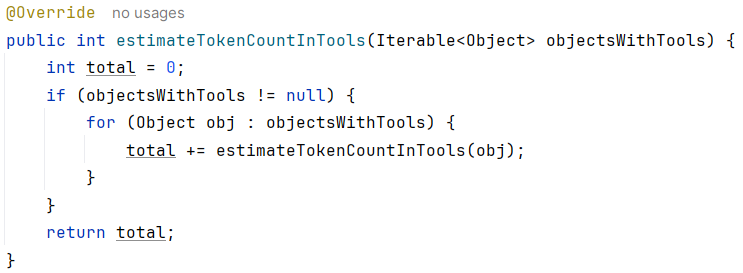
\includegraphics{before-stream.png}}
		\caption{\textit{Implémentation sans utiliser les Streams}}
		\label{fig:before-stream}
	\end{figure}
	
	Une évolution de cette implémentation utilisant les Streams ainsi que la bibliothèque Apache Commons est illustrée dans la figure \ref{fig:after-stream}.
	
	\begin{figure}[H]
		\centering
		\fbox{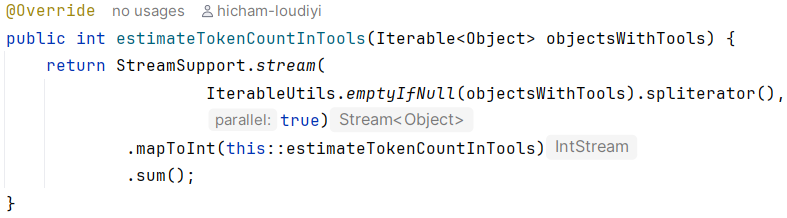
\includegraphics{after-stream.png}}
		\caption{\textit{Implémentation en utilisant les Streams}}
		\label{fig:after-stream}
	\end{figure}
	
	Cette implémentation, offrant une gestion robuste des null avec \verb|IterableUtils.emptyIfNull()|, convertit l'Iterable en Stream parallélisable avec \verb|StreamSupport.stream(..., true)|, ce qui permet un traitement réparti sur plusieurs cœurs CPU si la collection est grande, et une optimisation automatique pour les gros volumes de données, et finalement effectue un chaînage clair des opérations en appliquant les méthodes \verb|mapToInt(...)| et \verb|sum()|.
	
	\subsection{Importance de la factorisation du code}
	
	La factorisation du code consiste à regrouper dans des méthodes ou classes dédiées les portions de logique qui se répètent à plusieurs endroits du programme. Cette pratique s'inscrit dans les bonnes pratiques du développement logiciel, notamment le principe \textit{DRY} (\textit{Don't Repeat Yourself}), qui préconise d'éviter les duplications de code.
	
	Factoriser améliore la lisibilité, la maintenabilité, et réduit les risques d'erreurs en centralisant les modifications à un seul endroit. Cela permet également de clarifier les responsabilités des différentes classes, en accord avec le principe de responsabilité unique (\textit{Single Responsibility Principle}) du modèle SOLID.
	
	La figure \ref{fig:before-factorisation} montre une portion de code répétée avant factorisation.
	
	\begin{figure}[H]
		\centering
		\fbox{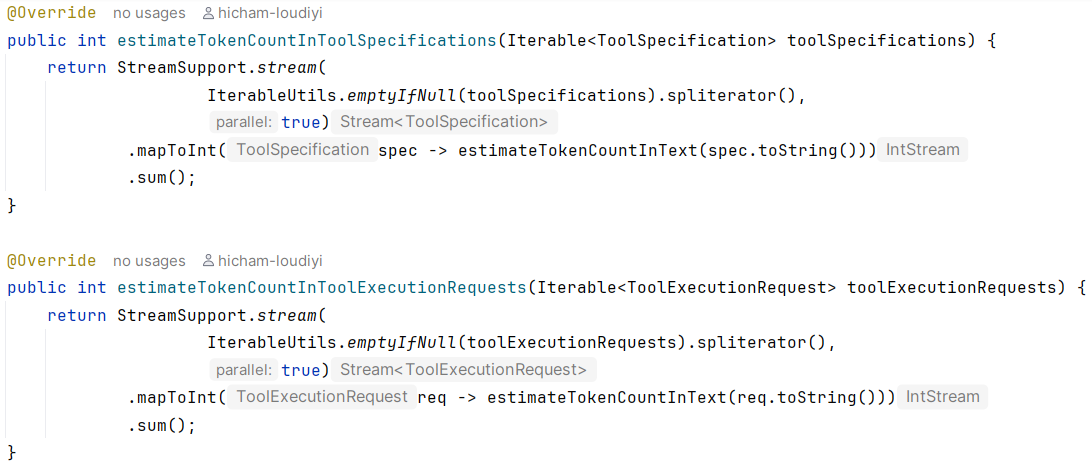
\includegraphics[width=1\textwidth]{before-factorisation.png}}
		\caption{\textit{Exemple de code répétitif avant factorisation}}
		\label{fig:before-factorisation}
	\end{figure}
	
	Dans la figure \ref{fig:before-factorisation}, chacune des méthodes \verb|estimateTokenCountInToolSpecifications| et \verb|estimateTokenCountInToolExecutionRequests| permet d'utiliser un Stream pour estimer un nombre de tokens sur un itérable, c'est donc une logique répétée, seuls le type d'objets de l'Iterable et la méthode de comptage appliquée à chaque objet sont différents. La figure \ref{fig:after-factorisation} illustre la version améliorée après factorisation.
	
	\begin{figure}[H]
		\centering
		\fbox{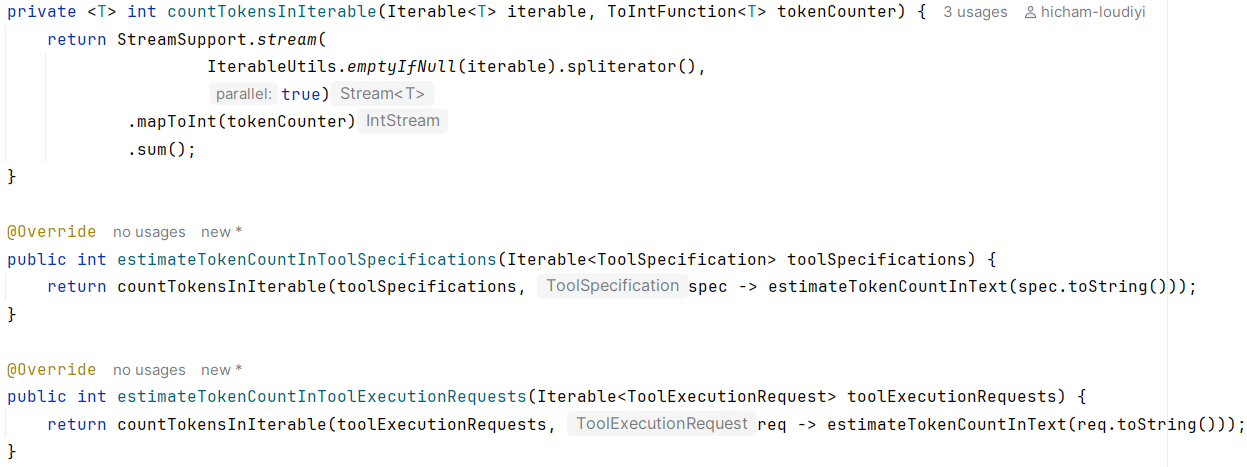
\includegraphics[width=1\textwidth]{after-factorisation.png}}
		\caption{\textit{Code refactorisé avec méthode utilitaire}}
		\label{fig:after-factorisation}
	\end{figure}
	
	La logique répétée est regroupée dans la méthode utilitaire \verb|countTokensInIterable|, puis réutilisée avec des appels dans les autres méthodes.
	
	On constate une nette amélioration de la clarté du code, les règles de validation sont centralisées dans une méthode dédiée, facilitant ainsi leur réutilisation et leur évolution future.
	
	
	
	
	\section{Premier prototype}
	
	\subsection{Introduction}
	
	Pour atteindre cet objectif ambitieux, nous avons suivi une approche incrémentale. Dans un premier temps, un prototype fonctionnel a été réalisé afin de valider les fondements techniques du projet. Ce prototype est une application basée sur un agent intelligent exploitant une architecture RAG (Retrieval-Augmented Generation), capable de répondre aux questions de l’utilisateur à partir d’un document texte ou PDF fourni. Cette première version a permis de :
	\begin{itemize}
		\item comprendre le fonctionnement du framework LangChain4j ;
		\item tester l’intégration avec le LLM Ollama ;
		\item valider le concept de récupération de contexte à partir de documents externes.
	\end{itemize}
	
	Pour tester ce prototype, nous avons fourni un fichier PDF, son contenu est une lettre de recommandation pour une étudiante appelée Nour, on a ensuite envoyé une question à propos de cette étudiante à l'agent AI, en utilisant un contrôleur web :
	
	\begin{figure}[H]
		\centering
		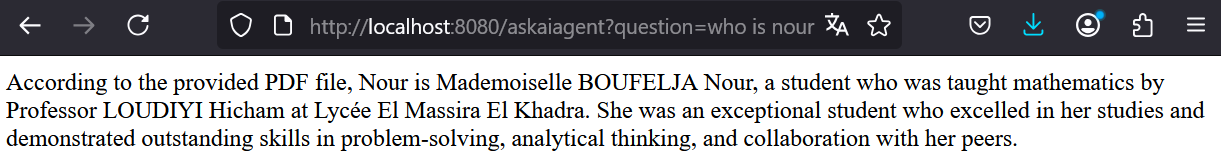
\includegraphics[width=\textwidth]{test-rag.png}
		\caption{\textit{Test du RAG}}
		\label{fig:test-rag}
	\end{figure}
	
	
	
\end{document}}